\documentclass[border=6pt]{standalone}
\usepackage{amsmath,amssymb}
\usepackage{tikz}
\begin{document}
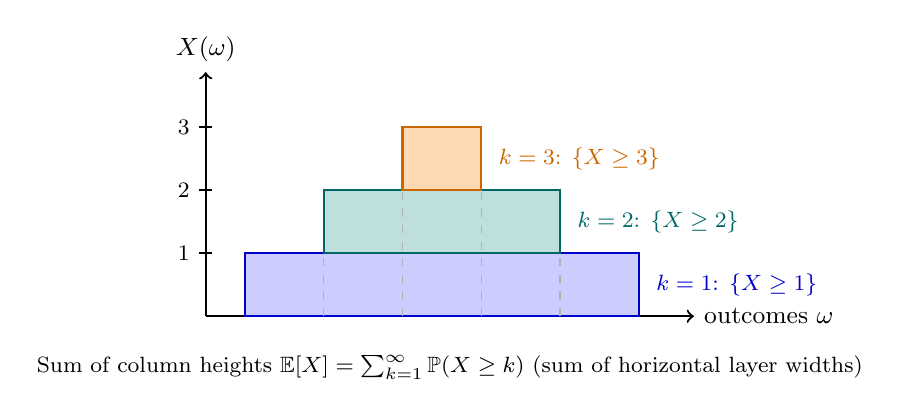
\begin{tikzpicture}[font=\small]
  \draw[->, thick] (0,0) -- (6.2,0) node[right] {outcomes $\omega$};
  \draw[->, thick] (0,0) -- (0,3.1) node[above] {$X(\omega)$};

  % Layer 1 (y from 0 to 0.8)
  \draw[fill=blue!20, draw=blue!80!black, thick] (0.5, 0) rectangle (5.5, 0.8);
  \node[right, blue!80!black] at (5.6, 0.4) {\footnotesize $k=1$: $\{X \ge 1\}$};

  % Layer 2 (y from 0.8 to 1.6)
  \draw[fill=teal!25, draw=teal!80!black, thick] (1.5, 0.8) rectangle (4.5, 1.6);
  \node[right, teal!80!black] at (4.6, 1.2) {\footnotesize $k=2$: $\{X \ge 2\}$};

  % Layer 3 (y from 1.6 to 2.4)
  \draw[fill=orange!30, draw=orange!80!black, thick] (2.5, 1.6) rectangle (3.5, 2.4);
  \node[right, orange!80!black] at (3.6, 2.0) {\footnotesize $k=3$: $\{X \ge 3\}$};

  % Subtle vertical dashed dividers showing the 5 discrete columns of heights 1, 2, 3, 2, 1
  \draw[dashed, gray!60] (1.5, 0) -- (1.5, 0.8);
  \draw[dashed, gray!60] (2.5, 0) -- (2.5, 1.6);
  \draw[dashed, gray!60] (3.5, 0) -- (3.5, 1.6);
  \draw[dashed, gray!60] (4.5, 0) -- (4.5, 0.8);

  % y-axis ticks and labels 1, 2, 3 at y = 0.8, 1.6, 2.4
  \foreach \y/\lbl in {0.8/1, 1.6/2, 2.4/3} {
    \draw[thick] (-0.08, \y) -- (0.08, \y);
    \node[left, font=\footnotesize] at (-0.08, \y) {$\lbl$};
  }

  \node[font=\footnotesize, align=center] at (3.1, -0.65)
    {Sum of column heights $\mathbb{E}[X] = \sum_{k=1}^\infty \mathbb{P}(X \ge k)$ (sum of horizontal layer widths)};
\end{tikzpicture}
\end{document}
